%%%%%%%%%%%%%%%%%%%%%%%%%%%%%%%%%%%%%%%%%
% Beamer Presentation
% LaTeX Template
% Version 1.0 (10/11/12)
%
% This template has been downloaded from:
% http://www.LaTeXTemplates.com
%
% License:
% CC BY-NC-SA 3.0 (http://creativecommons.org/licenses/by-nc-sa/3.0/)
%
%%%%%%%%%%%%%%%%%%%%%%%%%%%%%%%%%%%%%%%%%

%----------------------------------------------------------------------------------------
%	PACKAGES AND THEMES
%----------------------------------------------------------------------------------------

\documentclass[12pt]{beamer}

\mode<presentation>{

	% The Beamer class comes with a number of default slide themes
	% which change the colors and layouts of slides. Below this is a list
	% of all the themes, uncomment each in turn to see what they look like.

	%\usetheme{default}
	%\usetheme{AnnArbor}
	%\usetheme{Antibes}
	%\usetheme{Bergen}
	%\usetheme{Berkeley}
	%\usetheme{Berlin}
	%\usetheme{Boadilla}
	%\usetheme{CambridgeUS}
	%\usetheme{Copenhagen}
	%\usetheme{Darmstadt}
	%\usetheme{Dresden}
	%\usetheme{Frankfurt}
	%\usetheme{Goettingen}
	%\usetheme{Hannover}
	%\usetheme{Ilmenau}
	%\usetheme{JuanLesPins}
	%\usetheme{Luebeck}
	\usetheme{Madrid}
	%\usetheme{Malmoe}
	%\usetheme{Marburg}
	%\usetheme{Montpellier}
	%\usetheme{PaloAlto}
	%\usetheme{Pittsburgh}
	%\usetheme{Rochester}
	%\usetheme{Singapore}
	%\usetheme{Szeged}
	%\usetheme{Warsaw}

	% As well as themes, the Beamer class has a number of color themes
	% for any slide theme. Uncomment each of these in turn to see how it
	% changes the colors of your current slide theme.

	%\usecolortheme{albatross}
	%\usecolortheme{beaver}
	%\usecolortheme{beetle}
	%\usecolortheme{crane}
	%\usecolortheme{dolphin}
	%\usecolortheme{dove}
	%\usecolortheme{fly}
	%\usecolortheme{lily}
	%\usecolortheme{orchid}
	%\usecolortheme{rose}
	%\usecolortheme{seagull}
	\usecolortheme{seahorse}
	%\usecolortheme{whale}
	%\usecolortheme{wolverine}

	%\setbeamertemplate{footline} % To remove the footer line in all slides uncomment this line
	%\setbeamertemplate{footline}[page number] % To replace the footer line in all slides with a simple slide count uncomment this line

	%\setbeamertemplate{navigation symbols}{} % To remove the navigation symbols from the bottom of all slides uncomment this line
}

\usepackage{graphicx} % Allows including images
\usepackage{booktabs} % Allows the use of \toprule, \midrule and \bottomrule in tables

\usepackage[utf8]{inputenc}
\usepackage[ngerman]{babel}

\usepackage{ulem}
\usepackage{tikz}
\usetikzlibrary{arrows,shapes,positioning}


% lstlisting package

%==IMAGEPATH============================
\graphicspath{ {images/} }
%----------------------------------------------------
%==NEWCOMMAND=FOR=IMAGES============================
%img{\$name}{\$caption}{\$label}{\$witdh}
\newcommand{\img}[4] {
  \begin{figure}[H]
    \centering
    \includegraphics[width=#4\textwidth]{#1}
    \caption{#2}
    \label{fig:#3}
  \end{figure}}
%----------------------------------------------------

\usepackage{stmaryrd}
\usepackage{multirow}
\usepackage{amsmath}
\usepackage{listings}
\usepackage{lstautogobble}
\usepackage{wrapfig}
\definecolor{dkgreen}{rgb}{0,0.6,0}
\definecolor{gray}{rgb}{0.5,0.5,0.5}
\definecolor{mauve}{rgb}{0.58,0,0.82}
\lstset{
	%numbers = left,
	frame = single,
	basicstyle=\footnotesize, % the size of the fonts that are used for the code
	breakatwhitespace=false, % sets if automatic breaks should only happen at whitespace
	breaklines=true, % sets automatic line breaking
	captionpos=b, % sets the caption-position to bottom
	commentstyle=\color{dkgreen}, % comment style
	keywordstyle=\color{blue}, % keyword style
	%    language=C++, % the language of the code
	mathescape=true,
	basicstyle=\ttfamily\scriptsize,
autogobble}
\lstdefinelanguage{diff}{
	morecomment=[f][\color{blue}]{@@},     % group identifier
	morecomment=[f][\color{red}]-,         % deleted lines 
	morecomment=[f][\color{green}]+,       % added lines
	morecomment=[f][\color{magenta}]{---}, % Diff header lines (must appear after +,-)
	morecomment=[f][\color{magenta}]{+++},
}
%----------------------------------------------------------------------------------------
%	TITLE PAGE
%----------------------------------------------------------------------------------------

\title[Machine Learning -- ILP]{Inductive Logic Programming} % The short title appears at the bottom of every slide, the full title is only on the title page

\author{Christian Bay} % Your name
\institute[FAU] % Your institution as it will appear on the bottom of every slide, may be shorthand to save space
{
	FAU Erlangen-Nürnberg \\ % Your institution for the title page
	\medskip
	\textit{christian.bay@fau.de} % Your email address
}
\date{04.02.2016} % Date, can be changed to a custom date

\begin{document}

% Print Titlepage
\begin{frame}
	\titlepage
\end{frame}
\tableofcontents

\section{Grundlagen}

\frame{\frametitle{Agenda}\tableofcontents[currentsection]}
\begin{frame}
	\frametitle{Induction Logic Programming (ILP)}

	\begin{block}{Was ist Inductive Logic Programming?}
			Die Schnittstelle zwischen Machine Learning und logischer Programmierung
	\end{block}
	\img{process2cut}{Prozessablauf}{}{0.65}
\end{frame}

\begin{frame}
	\frametitle{Logik erster Stufe -- Einführung}

	In \textbf{Logik erster Stufe} besteht die Welt aus
	\begin{itemize}
		\item Objekten  $(Personen, Dingen)$
		\item Prädikaten $(>, <)$
		\item Funktionen $(+, -)$
	\end{itemize}
\end{frame}

\begin{frame}
	\frametitle{Logik erster Stufe -- Einführung}
	\emph{Terme} beschreiben Objekte in der Welt:\\
	\begin{itemize}
		\item Konstanten  ($2$, Chuck Norris)
		\item Variablen   ($x,y, a, \ldots$)
		\item Funktionen von Termen ($add(x,2)$)
	\end{itemize}

	\emph{Grundterme}: Terme ohne Variablen.
	\pause

	\vspace{15pt}
	\emph{Atome/Literale} sind kleinstmögliche Ausdrücke, die wahr/falsch sind
	\begin{itemize}
		\item $predicate(Term_1, \ldots, Term_n)$\\ 
			Beispiel: is\_human(Pinoccio)
		\item $Term_1 = Term_2$ (Gleicheitsrelation)
	\end{itemize}

\end{frame}

\begin{frame}
	\frametitle{Logik erster Stufe -- Syntax}

	\begin{block}{Syntaktische Beschreibung der Welt}
		\begin{align*}
			\text{Konstante} &= \{\text{Zero}\}\\
			\text{Funktion}  &=\{Succ/1, Plus/2 \}\\
			\text{Prädikate} &=\{even/1, is\_greater/2 \}
		\end{align*}
	\end{block}

\end{frame}

\begin{frame}
	\frametitle{Logik erster Stufe -- Semantik}
	Interpretation $\mathcal{I}$ besitzt eine Grundmenge $\mathcal{M}$
	und bildet Konstanten und Funktionen auf Elemente der Grundmenge ab.

	Prädikate werden auf Wahrheitswerte abgebildet

	\begin{block}{Interpretation}
		\begin{align*}
			\mathcal{M} &= \mathbb{N}_0\\
			\mathcal{I}(Zero) &= 0\\
			\mathcal{I}(Plus(Succ(Zero), Succ(Zero))) &= 2\\
			\mathcal{I}(even(Suc(Suc(Zero)))) &= True
		\end{align*}
	\end{block}
\end{frame}

\begin{frame}
	\frametitle{Logik erster Stufe -- Semantik II}
	\begin{block}{Logische Folgerung}
		Man schreibt
		\begin{align*}
			\Gamma \vDash \varphi
		\end{align*}
		Gdw. jede Intepretation $\mathcal{I}$, die alle Formeln
		der Menge $\Gamma$ erfüllt, auch $\varphi$ erfüllt.
	\end{block}
	\begin{bsp}
		\begin{align*}
			\{father(X,Y)\} \vDash father(\text{Darth Vader}, \text{Luke Skywalker})
		\end{align*}
	\end{bsp}
\end{frame}

\begin{frame}
	\frametitle{Horn-Klauseln}
	Horn Clauses: Klausel mit maximal einem positiven Literal.

	\begin{align*}
		\neg C_1 \lor \neg C_2 \lor \ldots \lor \neg C_n  \lor C_{n+1} \Leftrightarrow\\
		C_1 \land C_2 \land \ldots \land C_n  \rightarrow C_{n+1}
	\end{align*}

	ILP verwendet zumeist \textit{definite program clauses } (genau ein positives Literal) vom Typ:

	\begin{align*}
		\underbrace{T}_{\text{head}} \leftarrow \underbrace{L_1, \ldots, L_m}_{\text{body}}
	\end{align*}
	wobei $T, L_1, \ldots, L_m$ Literale sind, wobei $T$ immer positiv ist.

	Beispiel:
	\begin{align*}
		daughter(X,Y) \Leftarrow female(X), mother(Y, X)
	\end{align*}
\end{frame}

\begin{frame}
	\frametitle{Hypotheseneigenschaften}
	\emph{Gegeben:} Background-Knowledge $(\mathcal{B})$, Menge von positiven $(E^+)$ und negativen $(E^-)$ Beispielen\\
	\emph{Ziel:} Finden einer Hypothese $(\mathcal{H})$ die alle positiven und keine negativen
	Beispiele erfüllt

	\begin{minipage}{0.5\textwidth}
		\vspace{5pt}
		\underline{Eigenschaften}
		\begin{itemize}
			\item Sufficiency:        $\mathcal{B} \land \mathcal{H} \vDash E^{+}$

				Hypothese $\mathcal{H}$ muss alle positiven Beispiele logisch folgern

			\item Strong consistency: $\mathcal{B} \land \mathcal{H} \land E^{-} \nvDash false$

				$\mathcal{H}$ darf negativen Beispielen nicht widersprechen
		\end{itemize}
	\end{minipage}
	\begin{minipage}{0.45\textwidth}
		\centering
		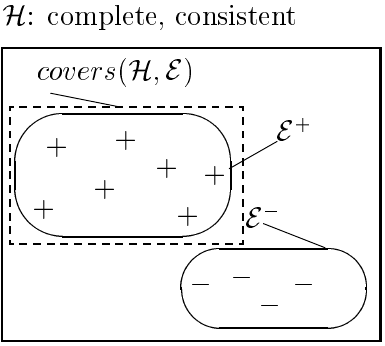
\includegraphics[scale=0.35]{hypothesis_correct}
	\end{minipage}
\end{frame}
%\begin{frame}
%\frametitle{Hypotheseneigenschaften}
%	\emph{Gegeben:} Background-Knowledge $(\mathcal{B})$, Menge von positiven $(E^+)$ und negativen $(E^-)$ Beispielen\\
%	\emph{Ziel:} Finden einer Hypothese $(\mathcal{H})$ die alle positiven und kein negatives Beispiele erfüllt
%\begin{figure}[H]
%	\centering
%	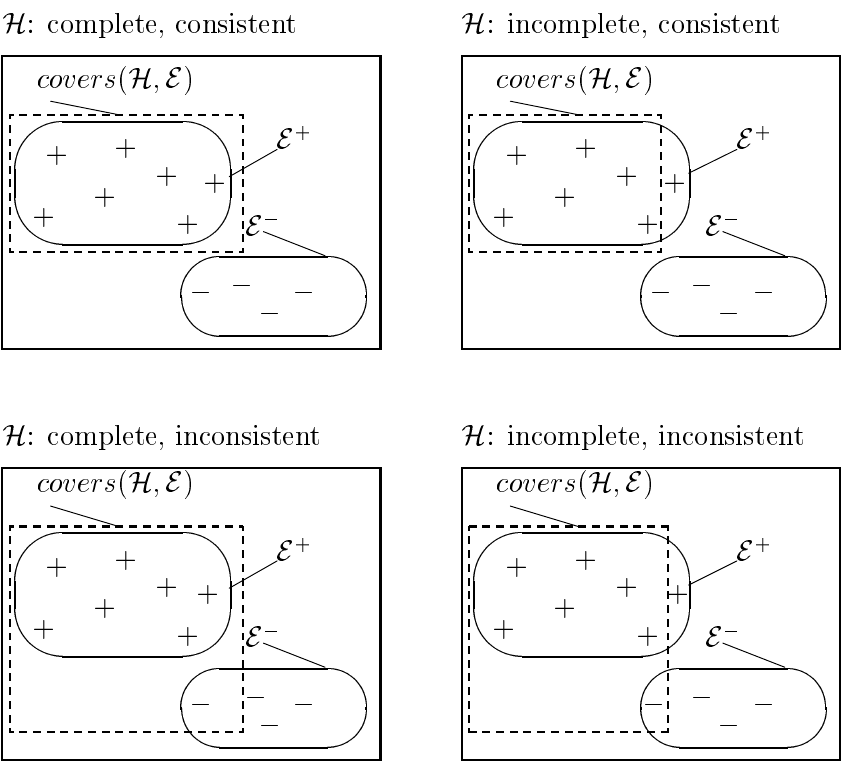
\includegraphics[width=0.5\textwidth]{hypothesis}
%\end{figure}
%\end{frame}
%
%\begin{frame}
%	\frametitle{Gewünschte Hypotheseneigenschaften}
%	\begin{itemize}
%		\item Necessity:          $\mathcal{B} \nvDash E^{+}$
%
%			Beispiele dürfen nicht durch Hintergrundwissen allein schon erklärbar sein
%
%		\item Sufficiency:        $\mathcal{B} \land \mathcal{H} \vDash E^{+}$
%
%			Hypothese $\mathcal{H}$ muss alle positiven Beispiele logisch folgern
%
%		\item Weak consistency:   $\mathcal{B} \land \mathcal{H} \nvDash false$
%
%			$\mathcal{H}$ darf dem Hintergrundwissen nicht widersprechen
%
%		\item Strong consistency: $\mathcal{B} \land \mathcal{H} \land E^{-} \nvDash false$
%
%			$\mathcal{H}$ darf negativen Beispielen nicht widersprechen
%	\end{itemize}
%\end{frame}

\section{Techniken des Inductive Logic Programming}
\frame{\frametitle{Agenda}\tableofcontents[currentsection]}
\subsection{Finden des Hypothesenraums}
\begin{frame}
	\frametitle{Subsumption von Literalen}
	\underline{Idee}: Eingrenzung des Suchraums erleichtert Hypothesensuche

	\begin{block}{Definition: Subsumption für Literale/Atome}
		Seien $L_1$ und $L_2$ Literale: $L_1 \underbrace{\preceq}_{\text{subsumiert}} L_2$
		wenn eine Substitution $\theta$ existert, sodass:
		\begin{align*}
			 L_1 \theta \subseteq L_2
		\end{align*}
	\end{block}
	\begin{bsp}
		\begin{align*}
			 daughter(X, Y)  \subseteq female(ann), daughter(mary, ann)\\\text{  mit  } \theta = \{X/mary, Y/ann\}
		\end{align*}
	\end{bsp}
\end{frame}
\begin{frame}
	\frametitle{Subsumption von Klauseln}
	Das gleiche Prozedere für Klauseln:
	\begin{block}{Definition: Subsumption für Klauseln}
		Seien $C_1$ und $C_2$ Klauseln: $C_1 \underbrace{\preceq}_{\text{subsumiert}} C_2$
		wenn eine Substitution $\theta$ existert, sodass:
		\begin{align*}
			 C_1 \theta \subseteq C_2
		\end{align*}
	\end{block}
	\begin{bsp}
		\begin{gather*}
			 daughter(X, Y) \leftarrow parent(Y,X) \subseteq\\
			 daughter(mary, ann) \leftarrow parent(ann, mary), parent(ann, tom)\\
			 \text{  mit  } \theta = \{X/mary, Y/ann\}
		\end{gather*}
	\end{bsp}
\end{frame}

\begin{frame}
	\frametitle{Eigenschaften der Subsumption}
	\begin{enumerate}
		\item {
			Wenn $C_1 \preceq C_2$ dann gilt (nicht umgekehrt!):
			\begin{align*}
				C_1 \vDash C_2
			\end{align*}
		}
		\item{ Die Relation $\leq$ führt ein Gitter (lattice) von reduzierten Klauseln ein
			\begin{figure}[H]
				\begin{center}
					\begin{tikzpicture}
						\node (G) at (1.5,2) {$\top$};
						\node (A) at (1.5,1.5) {$p(X,Y)$};
						\node (B) at (-1,0.5) {$p(X,a)$};
						\node (C) at (1.5,0.5) {$p(X,X)$};
						\node (D) at (4,0.5) {$p(a,Y)$};
						\node (E) at (1.5,-0.5) {$p(a,a)$};
						\node (F) at (1.5,-1) {$\bot$};
			
						\path [-] (A) edge node[left] {} (G);
						\path [-] (A) edge node[left] {} (B);
						\path [-] (A) edge node[left] {} (C);
						\path [-] (A) edge node[left] {} (D);
						\path [-] (B) edge node[left] {} (E);
						\path [-] (C) edge node[left] {} (E);
						\path [-] (D) edge node[left] {} (E);
						\path [-] (F) edge node[left] {} (E);
					\end{tikzpicture}
				\end{center}
				\caption{Partiell geordnete Menge von Formeln (POSET)}
				\label{fig:poset_atomic}
			\end{figure}
		}
	\end{enumerate}
\end{frame}

\subsection{Bottom-up -- Least general generalization}
\begin{frame}
	\frametitle{Least general generalization (LGG)}
	 Die \textit{least general generalization} von zwei Klauseln $C_1, C_2$ ist
	 die kleinste obere Schranke von $C_1,C_2$ im Gitter.

	\begin{block}{Erkenntnisse}
			\begin{itemize}
				\item [$\Rightarrow$] Alle Beispiele die $C_1$ abdeckt werden auch von
				allen 'kleineren Klauseln' abgedeckt
				\item[$\Rightarrow$] Wenn $C_1$ ein Beispiel nicht abdeckt,
				dann tut dies auch keine 'kleinere Klausel'
			\end{itemize}
	 \end{block}
\end{frame}

\begin{frame}
\frametitle{LGG - Algorithmus}
	\begin{block}{$lgg$ von Termen}
		\begin{enumerate}
			\item $lgg(t,t) = t$\\
			\item $lgg(f(s_1, \ldots, s_n), f(t_1, \ldots, t_n)) = f(lgg(s_1, t_1), \ldots, lgg(s_n, t_n))$
			\item Sonst: $lgg(t_1, t_2) = v , v$ freie Variable
		\end{enumerate}
	\end{block}
	\begin{block}{$lgg$ von Literalen}
	\begin{enumerate}
		\item $lgg(p(u_1, \ldots, u_n), p(s_1, \ldots, s_n)) = p(lgg(u_1, s_1), \ldots, lgg(u_n, s_n))$\\
		\item Sonst: $lgg(L_1, L_2) = \top$
	\end{enumerate}
	\end{block}
\end{frame}


\begin{frame}
\frametitle{RLGG - Algorithmus}
\begin{block}{Definition -- Relative least general generalization}
	Gegeben: Hintergrundwissen besteht nur aus \textit{ground literals} (Literale ohne Variablen).
	Sei $K$ die Konjunktion aller Hintergrundliterale und $e_1, e_2$ positive Beispiele
	\begin{align*}
		rlgg(e_1, e_2) = lgg((e_1 \leftarrow K), (e_2 \leftarrow K))
	\end{align*}
\end{block}

Beispiel: Familienkonstellation (siehe Terminal)
\img{family_relation}{Eine schrecklich nette Familie}{Familienrelation}{0.4}
\end{frame}


\begin{frame}{Linearity}
\frametitle{RLGG Anschaulich}
	\pgfdeclarelayer{background}
	\pgfsetlayers{background,main}
	\tikzstyle{vertex}=[rectangle,fill=black!25,minimum size=20pt,inner sep=0pt]
	\tikzstyle{selected vertex} = [vertex, fill=red!24]
	\tikzstyle{edge} = [draw,thick,-]
	\tikzstyle{weight} = [font=\small]
	\tikzstyle{selected edge} = [draw,line width=5pt,-,red!50]
	\setbeamercovered{invisible}
	\begin{figure}
		\begin{tikzpicture}[scale=1.0, auto,swap]
		\node[vertex] (a) at (0,0) {$A = e_1 \leftarrow K$};
		\node[vertex] (b) at (2.5,0) {$B = e_2 \leftarrow K$};
		\node[vertex] (c) at (5,0) {$C = e_3 \leftarrow K$};
		\node[vertex] (d) at (7.5,0) {$D = e_4 \leftarrow K$};\pause
		\node[vertex] (e) at (1.25,2) {$C' = lgg(A, B)$};
		\node[vertex] (f) at (6.25,2) {$C''= lgg(C, D)$};\pause
		\node[vertex] (g) at (3.75,4) {$\mathcal{H} = lgg(C', C'')$};
		\begin{pgfonlayer}{background}
			\path<2->[selected edge] (a.center) -- (e.center);
			\path<2->[selected edge] (b.center) -- (e.center);
			\path<2->[selected edge] (c.center) -- (f.center);
			\path<2->[selected edge] (d.center) -- (f.center);
			\path<3->[selected edge] (e.center) -- (g.center);
			\path<3->[selected edge] (f.center) -- (g.center);
		\end{pgfonlayer}
		\end{tikzpicture}
	\end{figure}
\end{frame}

\begin{frame}
	\frametitle{RLGG -- Algorithmus Erweitert}
	\begin{block}{Hintergrundwissen der Familienkonstellation}
		\begin{gather*}
			K = p(h,m), p(h,t), p(t,e), p(t,i), f(h), f(m), f(e)\\
			rlgg(e_1, e_2) = lgg((e_1 \leftarrow K), (e_2 \leftarrow K))
		\end{gather*}
	\end{block}

	Probleme: Große $\mathcal{H}$ bereits bei kleinen Beispielen:
	\begin{gather*}
		\begin{split}
			\underline{d(V_{m,e}, V_{h,t})} \leftarrow &\; p(h,m), p(h,t), p(t,e), p(t,i), f(h), f(m), f(e),\\
			&\; p(h, V_{m,t}), \underline{p(V_{h,t}, V_{m,e})}, p(V_{h,t}, V_{m,i}), p(V_{h,t}, V_{t,e}),\\
			&\; p(V_{h,t}, V_{t,i}) ,p(t, V_{e,i}), f(V_h, m), f(V_{h,e}), \underline{f(V_{m,e})}
		\end{split}
	\end{gather*}
\end{frame}

\begin{frame}
	\frametitle{RLGG -- Weiteres Probleme}
	\begin{itemize}
		\item $K$ bekommen wenn es nicht nur aus \textit{ground literals} besteht (Anhang: Saturierung)
		\item $\mathcal{H}$ kann nicht mehr als \emph{eine} Klausel umfassen
		\item Kombination der $lgg$-Paare bestimmt Qualität der Hypothese
	\end{itemize}
\end{frame}


\subsection{Bottom-up -- Inverse Resolution}
\begin{frame}
	\frametitle{Inverse resolution [Muggleton, Blutin '88]}
	Plotkins \textbf{LGG} Ansatz stark beschränkt

	Alternative Idee: \textbf{Inverse resolution}

	\begin{align*}
		B \wedge H \vDash E \Leftrightarrow\\
		B \wedge \neg E \vDash \neg H
	\end{align*}
	Suchen einer \textit{Bridgefunktion} $F$:
	\begin{align*}
		B \wedge \neg E \vDash F\\
		F \vDash \neg H\\
		\Rightarrow \neg F \Dashv H\\
		\Rightarrow \neg F \succeq H\\
	\end{align*}
\end{frame}


\begin{frame}
	\frametitle{Kurze Zwischenfrage}
	\img{wtf}{}{fig:wtf}{0.6}
\end{frame}

\begin{frame}
	\frametitle{Inverse resolution II}
	Generelle Idee: Laufe den Herleitungsbaum rückwärts

	\begin{block}{Herleitungsbaum Aussagenlogik}
		Sei Theorie $\mathcal{T}=\{ u \leftarrow v; v \leftarrow w, w\}$ gegeben.
		Herleitung von $u$:
		\begin{figure}[H]
			\begin{center}
				\begin{tikzpicture}[scale=0.6]
					\node (A) at (0.3, 0) {$u$};
					\node (B) at (-3.6,2.15) {$u \leftarrow v$};
					\node (C) at (-2,4) {$v \leftarrow w$};
					\node (D) at (2,4) {$w$};
					\node (E) at (1.3, 2.2) {$v$};

					\path [->] (B) edge node[above] {} (A);
					\path [->] (C) edge node[above] {} (E);
					\path [->] (D) edge node[above] {} (E);
					\path [->] (E) edge node[above] {} (A);
				\end{tikzpicture}
			\end{center}
		\end{figure}
	\end{block}
\end{frame}

\begin{frame}
	\frametitle{Inverse resolution III}
	Herleitungen in \textit{First order logic} benötigt zusätzlich Substitutionen:

	\begin{itemize}
		\item $\mathcal{H} = \{c\} = \{daugther(X,Y) \leftarrow female(X), parent(Y,X)\}$
		\item $\mathcal{B} = \{b_1, b_2\}$ mit $b_1 = female(mary)$ und
			$b_2 = parent(ann, mary)$
		\item $\mathcal{T} = \mathcal{B} \cup \mathcal{H}$
		\begin{figure}[H]
			\begin{center}
				\begin{tikzpicture}[scale=0.6]
					\node (A) at (0.3, 0) {\tiny{$daugher(mary,ann)$}};
					\node (B) at (-3.6,2.15) {\tiny{$b_2 = parent(ann,mary)$}};
					\node (C) at (-2,4) {\tiny{$b_1 = female(mary)$}};
					\node (D) at (2.5,5) {\tiny{$daughter(X,Y) \leftarrow female(X), parent(Y,X)$}};
					\node (E) at (1.3, 2.2) {\hspace{1cm}\tiny{$daughter(mary, Y) \leftarrow parent(Y,mary)$}};
					\node (S1) at (2.3, 1.2) {\tiny{$\theta_2 = \{Y/ann\}$}};
					\node (S1) at (3, 3.6) {\hspace{0.5cm}\tiny{$\theta_1 = \{X/mary\}$}};


					\path [->] (B) edge node[above] {} (A);
					\path [->] (C) edge node[above] {} (E);
					\path [->] (D) edge node[above] {} (E);
					\path [->] (E) edge node[above] {} (A);
				\end{tikzpicture}
			\end{center}
		\end{figure}
	\end{itemize}
\end{frame}

\begin{frame}
	\frametitle{Inverse resolution IV}
		Frage: Was bedeutet nun dieses \textbf{Inverse}?\\
		Antwort: Herleitung von $\mathcal{H}$ aus $\mathcal{E}$ und $\mathcal{B}$ mittels
		Inverse-Substitution

		\begin{block}{Beispiel: Inverse Substitution}
			Gegeben $c = daughter(X, Y) \leftarrow female(X), parent(Y,X)$ und
			die Substitution: $\theta = \{X/mary, Y/ann\}$
			\begin{align*}
				c' &= c\theta = daughter(mary, ann) \leftarrow female(mary), parent(ann, mary)\\
					c &= c'\theta^{-1} = daughter(X, Y) \leftarrow female(X), parent(Y,X)
			\end{align*}
		\end{block}
\end{frame}

\begin{frame}
	\frametitle{Inverse resolution V}
	Inverse resolution beginnt mit $\mathcal{H} = \{\} = \emptyset$

	\begin{itemize}
		\item $\mathcal{B} = \{b_1,b_2\}$ mit $b_1 = female(mary)$ und
			$b_2 = parent(ann, mary)$
		\item Positives Beispiel $e_1 = daughter(mary, ann)$
	\end{itemize}
\end{frame}

\begin{frame}
	\frametitle{Inverse resolution VI}
	Algorithmus:
	\begin{itemize}
		\item [1.] Finde Klausel $c_1$, sodass $\{b_2\} \cup c_1 \vDash e_1$
		\item [2.] Finde Klausel $c$, sodass $\{b_1\} \cup c \vDash c_1$
	\end{itemize}
		\begin{figure}[H]
			\begin{center}
				\begin{tikzpicture}[scale=0.8]
					\node (A) at (0.3, 0) {\tiny{$e_1 =daugher(mary,ann)$}};
					\node (B) at (-3.6,2.15) {\tiny{$b_2 = parent(ann,mary)$}};
					\node (C) at (-2,4) {\tiny{$b_1 = female(mary)$}};
					\node (D) at (2.5,5) {\tiny{$c = daughter(X,Y) \leftarrow female(X), parent(Y,X)$}};
					\node (E) at (1.3, 2.2) {\hspace{1cm}\tiny{$c_1 = daughter(mary, Y) \leftarrow parent(Y,mary)$}};
					\node (S1) at (2.3, 1.2) {\tiny{$\theta_2^{-1} = \{ann/Y\}$}};
					\node (S1) at (3, 3.6) {\hspace{0.5cm}\tiny{$\theta_1^{-1} = \{mary/X\}$}};


					\path [->] (B) edge node[above] {} (A);
					\path [->] (C) edge node[above] {} (E);
					\path [<-] (D) edge node[above] {} (E);
					\path [<-] (E) edge node[above] {} (A);
				\end{tikzpicture}
			\end{center}
		\end{figure}
\end{frame}

\begin{frame}
	\frametitle{Inverse resolution -- Zusammenfassung}
	Problem der \textit{Inverse resolution}:
	\begin{itemize}
		\item Nicht-deterministisch
		\item Hohe Komplexität (großer Suchraum)
		\item Gegenstand der aktuellen Forschung
	\end{itemize}
\end{frame}

\subsection{Top-down -- Refinement-Operator}
\begin{frame}[fragile]
\frametitle{Top-Down Ansatz}
Idee: Klauseln zu immer weiter spezifizieren

\begin{enumerate}
	\item Beginne mit Prädikat von dem Beispiele gebaut sind
	\item Füge solange Literale in Header hinzu, bis passende Beispiele erfüllt sind.
\end{enumerate}



	\begin{block}{Der Refinement-Operator $\rho$ [Shapiro '83]}
\begin{align*}
	\forall D \in \rho(C). C \preceq D
\end{align*}
	Gewünschte Eigenschaften:
	\begin{itemize}
		\item \textit{Finite}: Erhalte endliche Menge an Klauseln
		\item \textit{Complete}: Generierung aller subsummierenden Klauseln
		\item \textit{Non-redundant}: Jede Klausel kann nur auf einen Weg generiert werden
			(Vernachlässigbar)
	\end{itemize}
\end{block}
\end{frame}

\begin{frame}
\frametitle{Refinement-Operator}
Beispiel für $\rho$:
\begin{figure}[H]
	\begin{center}
		\begin{tikzpicture}[scale=0.93]
			\node (A) at (1.5,1) {$p(X,Y)$};
			\node (B) at (-3,-1) {$p(X,X)$};
			\node (C) at (0,-1) {$p(f(Z_1,Z_2), Y)$};
			\node (D) at (3,-1) {$p(X,f(Z_1,Z_2))$};
			\node (E) at (7,-1) {$p(X,Y) \leftarrow q(Z_1, Z_2)$};

			\path [->] (A) edge node[above] {op2} (B);
			\path [->] (A) edge node[right] {op1} (C);
			\path [->] (A) edge node[right] {op1} (D);
			\path [->] (A) edge node[above] {op3} (E);
		\end{tikzpicture}
	\end{center}
	\caption{Beispiel für einen refinement-operator}
	\label{fig:refinement_operator}
\end{figure}
\end{frame}

\begin{frame}
	\frametitle{Familienkonstellation: Top-Down}
	\begin{figure}[H]
		\begin{center}
			\begin{tikzpicture}[scale=1.0]
				\node[font=\tiny] (A) at (1.5,1) {$daughter(X,Y)\leftarrow$};
				\node[font=\tiny] (B) at (-1,0) {$daughter(X,Y) \leftarrow X = Y$};
				\node[font=\tiny] (C) at (0,-1) {$daughter(X,Y) \leftarrow female(X)$};
				\node[font=\tiny] (D) at (2.5,-0.5) {$daughter(X,Y) \leftarrow parent(Y,X)$};
				\node[font=\tiny] (E) at (4.5,0) {$daughter(X,Y) \leftarrow parent(X, Z)$};
				\node[font=\tiny] (F) at (-2,-1.75) {$daughter(X,Y)\leftarrow female(X), female(Y)$};
				\node[font=\tiny] (G) at (2.75, -1.75) {$daughter(X,Y) \leftarrow female(X), parent(Y,X)$};
				\node[font=\tiny] (X) at (1.35, -0) {$\ldots$};
				\node[font=\tiny] (Y) at (0.3, -1.5) {$\ldots$};
	
				\path [->] (A) edge node[left] {} (B);
				\path [->] (A) edge node[left] {} (C);
				\path [->] (A) edge node[left] {} (D);
				\path [->] (A) edge node[left] {} (E);
				\path [->] (C) edge node[left] {} (F);
				\path [->] (C) edge node[left] {} (G);
			\end{tikzpicture}
		\end{center}
		\caption{Teil des Refinementgraphs für Familienkonstellation}
		\label{fig:refinement_operator}
	\end{figure}
	\begin{block}{Refinement-Operator}
		$\rho(c) = \{daughter(X, Y) \leftarrow L\}$\\
	\end{block}
\end{frame}

\begin{frame}
	\frametitle{Top-Down - Varianten}
	Wie durchsucht man den Refinementgraph?
	\begin{itemize}
		\item Variante 1: Vollständig (ggf langsam)
		\item Variante 2: Greedy (ggf unvollständig)
	\end{itemize}
	\begin{block}{Verbesserung von Top-Down}
		Verkleinere Suchraum durch Seed
	\end{block}
	\begin{center}
	\begin{tikzpicture}
				\node[font=\tiny] (A) at (1.5,1) {$p(X,Y)$};
				\node[font=\tiny] (B) at (-1,0) {$p(X,X)$};
				\node[font=\tiny] (C) at (0.55,0) {$p(X,Y) \leftarrow r(U)$};
				\node[font=\tiny] (D) at (2.6,0) {$p(X,Y) \leftarrow q(V)$};
				\node[font=\tiny] (E) at (1.5,-2) {$p(X,Y) \leftarrow r(X), q(X), q(Y)$};
				\node[font=\tiny] (X) at (1.75, 0.5) {$\ldots$};
				\node[font=\tiny] (Y) at (0.6, 0.5) {$\ldots$};
				\node[font=\tiny] (B2) at (0.3,-1.3)  {};
				\node[font=\tiny] (C2) at (1.5,-1) {};
				\node[font=\tiny] (D2) at (3,-1.3) {};
				\node[font=\tiny] (B3) at (-1,-1.5) {\ldots};
				\node[font=\tiny] (D3) at (4,-1.5) {\ldots};
				\node[font=\tiny] (X2) at (1, -1.25) {$\ldots$};
				\node[font=\tiny] (Y2) at (2, -1.25) {$\ldots$};
	
				\path [->] (A) edge node[left] {} (B);
				\path [->] (A) edge node[left] {} (C);
				\path [->] (A) edge node[left] {} (D);
				\path [->] (B2) edge node[left] {} (E);
				\path [->] (C2) edge node[left] {} (E);
				\path [->] (D2) edge node[left] {} (E);
		\begin{scope}[label distance=0mm,]
			\coordinate  (aux1) at ([yshift=-15pt]A);
			\coordinate  (aux2) at ([yshift=+10pt]E);
			\node[regular polygon,regular polygon sides=5,draw, red,fit={(aux1) (aux2)},label=right:{\color{red}\small{Bereich mit Seed}}] {};
		\end{scope}
		%\begin{scope}[label distance=6mm,]
		%	\foreach \i/\label in {1/Label 1,2/Label 2,3/Label 3}
		%	{
		%		  \coordinate  (aux\i) at ([xshift=2cm]t\i);
		%		    \node[inner sep=6pt,rounded corners=6pt,draw,red,fit={(t\i) (b\i)
		%			(aux\i)},label=right:{\color{red}\label}] {};
		%			}
		%\end{scope}
	\end{tikzpicture}
	\end{center}
\end{frame}

\section{Anwendungsgebiete}
\frame{\frametitle{Agenda}\tableofcontents[currentsection]}
\subsection{QSAR}
\begin{frame}
	\frametitle{Quantitative structure-activity relationships}
	Problemstellung aus \textbf{Pharmazie}: Stoffe entwickeln mit speziellen biologische Eigenschaften.
	Welche Restgruppenkombination führt zu gewünschten Eigenschaften?\\

	Restgruppen ($OH, F, Br, NH_2, No_2, \ldots)$ haben verschiedene
	chemisch-physikalische Eigenschaften
	\begin{itemize}
		\item Polarität
		\item Größe
		\item Symmetrie
		\item Basisch, sauer
		\item {\hspace{5pt}\vdots}
	\end{itemize}
\end{frame}
\begin{frame}
	\frametitle{Quantitative structure-activity relationships}
	\begin{block}{Beispiel: Thrimethoprim}
		\img{qsar}{Trimethoprim mit Restgruppen}{fig:trim}{0.6}
	\end{block}
	Welche Restgruppenkombination führt zu welchen biologischen Eigenschaften?
\end{frame}
\begin{frame}[fragile]
	\frametitle{Quantitative structure-activity relationships}
	Standard Verfahren nach \textit{Hansch}: Vorhersage durch Bildung von
	Gleichungssystem über phy.-chem. Eigenschaften der Restgruppen

	\begin{block}{ILP-Ansatz}
	Hintergrundwissen erstellen durch bereits bekannte biologische Eigenschaften
	von Stoffen.
	\begin{itemize}
		\item Jeder Restgryppe Eigenschaften zuweisen: $polar(NO_2, polar\_value), \ldots$
		\item $great(DrugX, DrugY)$: $X$ hat höhere biologische Aktivität als $Y$
		\item Regeln für $great(A,B)$ erstellen: 
			\begin{lstlisting}[language=prolog]
				great(A,B) $\leftarrow$ struc(A,D,E,F), struc(B,h,C,h), flex(D,G),
				less_4_flex(G), h_donor(D, h_don_0), pi(D, po_don_1).
			\end{lstlisting}
	\end{itemize}
	\end{block}
\end{frame}

\begin{frame}
	\frametitle{Quantitative structure-activity relationships}
	Bewertung:
	\begin{center}
		\begin{tabular}{|c|c|c|}
			\hline
			& ILP & Hansch\\
			\hline
			Korrelation Training & 0.92 & 0.79\\
			\hline
			Korrelation Test     & 0.46 -- 0.54 & 0.42\\
			\hline
		\end{tabular}
		\captionof{table}{Korelationstabelle für QSAR}
		\end{center}
		Erkenntnis:\\
		ILP funktioniert gut solange Moleküle nicht zu komplex sind.
\end{frame}

\begin{frame}
	\frametitle{Weitere Real-World Anwendungen}
	Weitere Anwendungen in Real-World:
	\begin{itemize}
		\item Sekundäre Protein Struktur vorhersagen
		\item Regeln für Rheuma Früherkennung finden
	\end{itemize}
\end{frame}

\section{Zusammenfassung}
\frame{\frametitle{Agenda}\tableofcontents[currentsection]}
\begin{frame}
	\frametitle{Zusammenfassung}
	Weitere Anwendungen in Real-World:
	Bedingungen für ILP:
	\begin{itemize}
		\item \textbf{Formalierbarkeit} von Problemen
		\item Überschaubare Komplexität
		\item Je nach Problem sind ILP-Systeme besser/schlechter geeignet
	\end{itemize}
\end{frame}

\section{Quellen}
\begin{frame}[allowframebreaks]{Quellen}
    \raggedright
    \nocite{*}
    \bibliographystyle{plain}
    \bibliography{ref}
\end{frame}

\end{document}
